\chapter{The Telegraph}

M. and Madame de Villefort found on their return that the Count of
Monte Cristo, who had come to visit them in their absence, had been
ushered into the drawing-room, and was still awaiting them there.
Madame de Villefort, who had not yet sufficiently recovered from her
late emotion to allow of her entertaining visitors so immediately,
retired to her bedroom, while the procureur, who could better depend
upon himself, proceeded at once to the salon.

Although M. de Villefort flattered himself that, to all outward view,
he had completely masked the feelings which were passing in his mind,
he did not know that the cloud was still lowering on his brow, so much
so that the count, whose smile was radiant, immediately noticed his
sombre and thoughtful air.

“\textit{Ma foi!}” said Monte Cristo, after the first compliments were over,
“what is the matter with you, M. de Villefort? Have I arrived at the
moment when you were drawing up an indictment for a capital crime?”

Villefort tried to smile.

“No, count,” he replied, “I am the only victim in this case. It is I
who lose my cause, and it is ill-luck, obstinacy, and folly which have
caused it to be decided against me.”

“To what do you refer?” said Monte Cristo with well-feigned interest.
“Have you really met with some great misfortune?”

“Oh, no, monsieur,” said Villefort with a bitter smile; “it is only a
loss of money which I have sustained—nothing worth mentioning, I assure
you.”

“True,” said Monte Cristo, “the loss of a sum of money becomes almost
immaterial with a fortune such as you possess, and to one of your
philosophic spirit.”

“It is not so much the loss of the money that vexes me,” said
Villefort, “though, after all, 900,000 francs are worth regretting; but
I am the more annoyed with this fate, chance, or whatever you please to
call the power which has destroyed my hopes and my fortune, and may
blast the prospects of my child also, as it is all occasioned by an old
man relapsed into second childhood.”

\begin{figure}[ht]
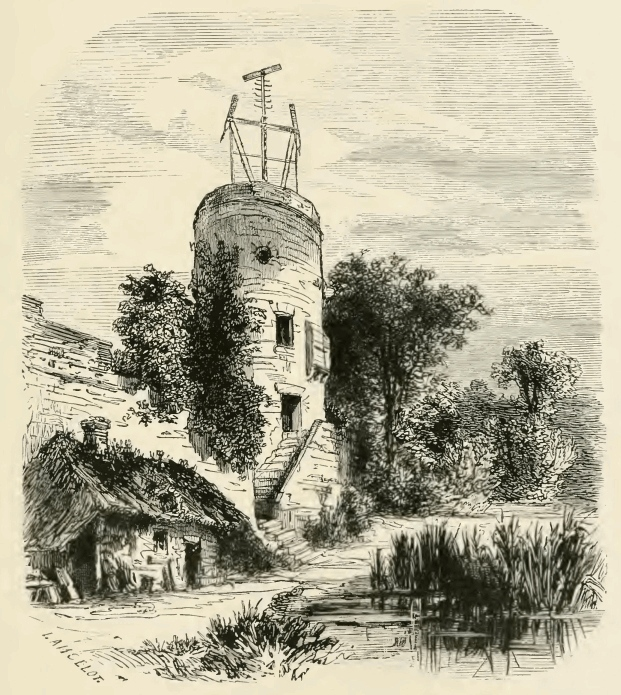
\includegraphics[width=\textwidth]{30183m.jpg}
\end{figure}

“What do you say?” said the count; “900,000 francs? It is indeed a sum
which might be regretted even by a philosopher. And who is the cause of
all this annoyance?”

“My father, as I told you.”

“M. Noirtier? But I thought you told me he had become entirely
paralyzed, and that all his faculties were completely destroyed?”

“Yes, his bodily faculties, for he can neither move nor speak,
nevertheless he thinks, acts, and wills in the manner I have described.
I left him about five minutes ago, and he is now occupied in dictating
his will to two notaries.”

“But to do this he must have spoken?”

“He has done better than that—he has made himself understood.”

“How was such a thing possible?”

“By the help of his eyes, which are still full of life, and, as you
perceive, possess the power of inflicting mortal injury.”

“My dear,” said Madame de Villefort, who had just entered the room,
“perhaps you exaggerate the evil.”

“Good-morning, madame,” said the count, bowing.

Madame de Villefort acknowledged the salutation with one of her most
gracious smiles.

“What is this that M. de Villefort has been telling me?” demanded Monte
Cristo “and what incomprehensible misfortune——”

“Incomprehensible is the word!” interrupted the procureur, shrugging
his shoulders. “It is an old man’s caprice!”

“And is there no means of making him revoke his decision?”

“Yes,” said Madame de Villefort; “and it is still entirely in the power
of my husband to cause the will, which is now in prejudice of
Valentine, to be altered in her favor.”

The count, who perceived that M. and Madame de Villefort were beginning
to speak in parables, appeared to pay no attention to the conversation,
and feigned to be busily engaged in watching Edward, who was
mischievously pouring some ink into the bird’s water-glass.

“My dear,” said Villefort, in answer to his wife, “you know I have
never been accustomed to play the patriarch in my family, nor have I
ever considered that the fate of a universe was to be decided by my
nod. Nevertheless, it is necessary that my will should be respected in
my family, and that the folly of an old man and the caprice of a child
should not be allowed to overturn a project which I have entertained
for so many years. The Baron d’Épinay was my friend, as you know, and
an alliance with his son is the most suitable thing that could possibly
be arranged.”

“Do you think,” said Madame de Villefort, “that Valentine is in league
with him? She has always been opposed to this marriage, and I should
not be at all surprised if what we have just seen and heard is nothing
but the execution of a plan concerted between them.”

“Madame,” said Villefort, “believe me, a fortune of 900,000 francs is
not so easily renounced.”

“She could, nevertheless, make up her mind to renounce the world, sir,
since it is only about a year ago that she herself proposed entering a
convent.”

“Never mind,” replied Villefort; “I say that this marriage \textit{shall} be
consummated.”

“Notwithstanding your father’s wishes to the contrary?” said Madame de
Villefort, selecting a new point of attack. “That is a serious thing.”

Monte Cristo, who pretended not to be listening, heard however, every
word that was said.

\begin{figure}[ht]
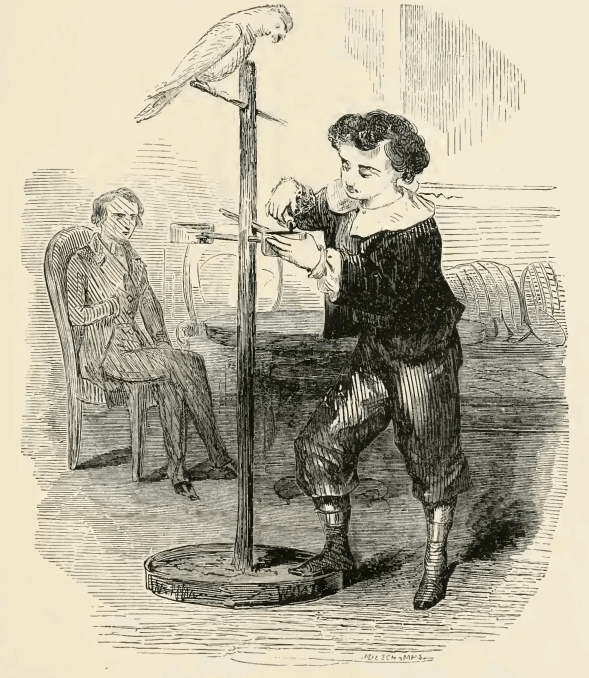
\includegraphics[width=\textwidth]{30185m.jpg}
\end{figure}

“Madame,” replied Villefort “I can truly say that I have always
entertained a high respect for my father, because, to the natural
feeling of relationship was added the consciousness of his moral
superiority. The name of father is sacred in two senses; he should be
reverenced as the author of our being and as a master whom we ought to
obey. But, under the present circumstances, I am justified in doubting
the wisdom of an old man who, because he hated the father, vents his
anger on the son. It would be ridiculous in me to regulate my conduct
by such caprices. I shall still continue to preserve the same respect
toward M. Noirtier; I will suffer, without complaint, the pecuniary
deprivation to which he has subjected me; but I shall remain firm in my
determination, and the world shall see which party has reason on his
side. Consequently I shall marry my daughter to the Baron Franz
d’Épinay, because I consider it would be a proper and eligible match
for her to make, and, in short, because I choose to bestow my
daughter’s hand on whomever I please.”

“What?” said the count, the approbation of whose eye Villefort had
frequently solicited during this speech. “What? Do you say that M.
Noirtier disinherits Mademoiselle de Villefort because she is going to
marry M. le Baron Franz d’Épinay?”

“Yes, sir, that is the reason,” said Villefort, shrugging his
shoulders.

“The apparent reason, at least,” said Madame de Villefort.

“The \textit{real} reason, madame, I can assure you; I know my father.”

“But I want to know in what way M. d’Épinay can have displeased your
father more than any other person?”

“I believe I know M. Franz d’Épinay,” said the count; “is he not the
son of General de Quesnel, who was created Baron d’Épinay by Charles
X.?”

“The same,” said Villefort.

“Well, but he is a charming young man, according to my ideas.”

“He is, which makes me believe that it is only an excuse of M. Noirtier
to prevent his granddaughter marrying; old men are always so selfish in
their affection,” said Madame de Villefort.

“But,” said Monte Cristo “do you not know any cause for this hatred?”

“Ah, \textit{ma foi!} who is to know?”

“Perhaps it is some political difference?”

“My father and the Baron d’Épinay lived in the stormy times of which I
only saw the ending,” said Villefort.

“Was not your father a Bonapartist?” asked Monte Cristo; “I think I
remember that you told me something of that kind.”

“My father has been a Jacobin more than anything else,” said Villefort,
carried by his emotion beyond the bounds of prudence; “and the
senator’s robe, which Napoleon cast on his shoulders, only served to
disguise the old man without in any degree changing him. When my father
conspired, it was not for the emperor, it was against the Bourbons; for
M. Noirtier possessed this peculiarity, he never projected any Utopian
schemes which could never be realized, but strove for possibilities,
and he applied to the realization of these possibilities the terrible
theories of The Mountain,—theories that never shrank from any means
that were deemed necessary to bring about the desired result.”

“Well,” said Monte Cristo, “it is just as I thought; it was politics
which brought Noirtier and M. d’Épinay into personal contact. Although
General d’Épinay served under Napoleon, did he not still retain
royalist sentiments? And was he not the person who was assassinated one
evening on leaving a Bonapartist meeting to which he had been invited
on the supposition that he favored the cause of the emperor?”

Villefort looked at the count almost with terror.

“Am I mistaken, then?” said Monte Cristo.

“No, sir, the facts were precisely what you have stated,” said Madame
de Villefort; “and it was to prevent the renewal of old feuds that M.
de Villefort formed the idea of uniting in the bonds of affection the
two children of these inveterate enemies.”

“It was a sublime and charitable thought,” said Monte Cristo, “and the
whole world should applaud it. It would be noble to see Mademoiselle
Noirtier de Villefort assuming the title of Madame Franz d’Épinay.”

Villefort shuddered and looked at Monte Cristo as if he wished to read
in his countenance the real feelings which had dictated the words he
had just uttered. But the count completely baffled the procureur, and
prevented him from discovering anything beneath the never-varying smile
he was so constantly in the habit of assuming.

“Although,” said Villefort, “it will be a serious thing for Valentine
to lose her grandfather’s fortune, I do not think that M. d’Épinay will
be frightened at this pecuniary loss. He will, perhaps, hold me in
greater esteem than the money itself, seeing that I sacrifice
everything in order to keep my word with him. Besides, he knows that
Valentine is rich in right of her mother, and that she will, in all
probability, inherit the fortune of M. and Madame de Saint-Méran, her
mother’s parents, who both love her tenderly.”

“And who are fully as well worth loving and tending as M. Noirtier,”
said Madame de Villefort; “besides, they are to come to Paris in about
a month, and Valentine, after the affront she has received, need not
consider it necessary to continue to bury herself alive by being shut
up with M. Noirtier.”

The count listened with satisfaction to this tale of wounded self-love
and defeated ambition.

“But it seems to me,” said Monte Cristo, “and I must begin by asking
your pardon for what I am about to say, that if M. Noirtier disinherits
Mademoiselle de Villefort because she is going to marry a man whose
father he detested, he cannot have the same cause of complaint against
this dear Edward.”

“True,” said Madame de Villefort, with an intonation of voice which it
is impossible to describe; “is it not unjust—shamefully unjust? Poor
Edward is as much M. Noirtier’s grandchild as Valentine, and yet, if
she had not been going to marry M. Franz, M. Noirtier would have left
her all his money; and supposing Valentine to be disinherited by her
grandfather, she will still be three times richer than he.”

The count listened and said no more.

“Count,” said Villefort, “we will not entertain you any longer with our
family misfortunes. It is true that my patrimony will go to endow
charitable institutions, and my father will have deprived me of my
lawful inheritance without any reason for doing so, but I shall have
the satisfaction of knowing that I have acted like a man of sense and
feeling. M. d’Épinay, to whom I had promised the interest of this sum,
shall receive it, even if I endure the most cruel privations.”

“However,” said Madame de Villefort, returning to the one idea which
incessantly occupied her mind, “perhaps it would be better to explain
this unlucky affair to M. d’Épinay, in order to give him the
opportunity of himself renouncing his claim to the hand of Mademoiselle
de Villefort.”

“Ah, that would be a great pity,” said Villefort.

“A great pity,” said Monte Cristo.

“Undoubtedly,” said Villefort, moderating the tones of his voice, “a
marriage once concerted and then broken off, throws a sort of discredit
on a young lady; then again, the old reports, which I was so anxious to
put an end to, will instantly gain ground. No, it will all go well; M.
d’Épinay, if he is an honorable man, will consider himself more than
ever pledged to Mademoiselle de Villefort, unless he were actuated by a
decided feeling of avarice, but that is impossible.”

“I agree with M. de Villefort,” said Monte Cristo, fixing his eyes on
Madame de Villefort; “and if I were sufficiently intimate with him to
allow of giving my advice, I would persuade him, since I have been told
M. d’Épinay is coming back, to settle this affair at once beyond all
possibility of revocation. I will answer for the success of a project
which will reflect so much honor on M. de Villefort.”

The procureur arose, delighted with the proposition, but his wife
slightly changed color.

“Well, that is all that I wanted, and I will be guided by a counsellor
such as you are,” said he, extending his hand to Monte Cristo.
“Therefore let everyone here look upon what has passed today as if it
had not happened, and as though we had never thought of such a thing as
a change in our original plans.”

“Sir,” said the count, “the world, unjust as it is, will be pleased
with your resolution; your friends will be proud of you, and M.
d’Épinay, even if he took Mademoiselle de Villefort without any dowry,
which he will not do, would be delighted with the idea of entering a
family which could make such sacrifices in order to keep a promise and
fulfil a duty.”

At the conclusion of these words, the count rose to depart.

“Are you going to leave us, count?” said Madame de Villefort.

“I am sorry to say I must do so, madame, I only came to remind you of
your promise for Saturday.”

“Did you fear that we should forget it?”

“You are very good, madame, but M. de Villefort has so many important
and urgent occupations.”

“My husband has given me his word, sir,” said Madame de Villefort; “you
have just seen him resolve to keep it when he has everything to lose,
and surely there is more reason for his doing so where he has
everything to gain.”

“And,” said Villefort, “is it at your house in the Champs-Élysées that
you receive your visitors?”

“No,” said Monte Cristo, “which is precisely the reason which renders
your kindness more meritorious,—it is in the country.”

“In the country?”

“Yes.”

“Where is it, then? Near Paris, is it not?”

“Very near, only half a league from the Barriers,—it is at Auteuil.”

“At Auteuil?” said Villefort; “true, Madame de Villefort told me you
lived at Auteuil, since it was to your house that she was taken. And in
what part of Auteuil do you reside?”

“Rue de la Fontaine.”

“Rue de la Fontaine!” exclaimed Villefort in an agitated tone; “at what
number?”

“No. 28.”

“Then,” cried Villefort, “was it you who bought M. de Saint-Méran’s
house!”

“Did it belong to M. de Saint-Méran?” demanded Monte Cristo.

“Yes,” replied Madame de Villefort; “and, would you believe it,
count——”

“Believe what?”

“You think this house pretty, do you not?”

“I think it charming.”

“Well, my husband would never live in it.”

“Indeed?” returned Monte Cristo, “that is a prejudice on your part, M.
de Villefort, for which I am quite at a loss to account.”

“I do not like Auteuil, sir,” said the procureur, making an evident
effort to appear calm.

“But I hope you will not carry your antipathy so far as to deprive me
of the pleasure of your company, sir,” said Monte Cristo.

“No, count,—I hope—I assure you I shall do my best,” stammered
Villefort.

“Oh,” said Monte Cristo, “I allow of no excuse. On Saturday, at six
o’clock. I shall be expecting you, and if you fail to come, I shall
think—for how do I know to the contrary?—that this house, which has
remained uninhabited for twenty years, must have some gloomy tradition
or dreadful legend connected with it.”

“I will come, count,—I will be sure to come,” said Villefort eagerly.

“Thank you,” said Monte Cristo; “now you must permit me to take my
leave of you.”

“You said before that you were obliged to leave us, monsieur,” said
Madame de Villefort, “and you were about to tell us why when your
attention was called to some other subject.”

“Indeed madame,” said Monte Cristo: “I scarcely know if I dare tell you
where I am going.”

“Nonsense; say on.”

“Well, then, it is to see a thing on which I have sometimes mused for
hours together.”

“What is it?”

“A telegraph. So now I have told my secret.”

“A telegraph?” repeated Madame de Villefort.

“Yes, a telegraph. I had often seen one placed at the end of a road on
a hillock, and in the light of the sun its black arms, bending in every
direction, always reminded me of the claws of an immense beetle, and I
assure you it was never without emotion that I gazed on it, for I could
not help thinking how wonderful it was that these various signs should
be made to cleave the air with such precision as to convey to the
distance of three hundred leagues the ideas and wishes of a man sitting
at a table at one end of the line to another man similarly placed at
the opposite extremity, and all this effected by a simple act of
volition on the part of the sender of the message. I began to think of
genii, sylphs, gnomes, in short, of all the ministers of the occult
sciences, until I laughed aloud at the freaks of my own imagination.
Now, it never occurred to me to wish for a nearer inspection of these
large insects, with their long black claws, for I always feared to find
under their stone wings some little human genius fagged to death with
cabals, factions, and government intrigues. But one fine day I learned
that the mover of this telegraph was only a poor wretch, hired for
twelve hundred francs a year, and employed all day, not in studying the
heavens like an astronomer, or in gazing on the water like an angler,
or even in enjoying the privilege of observing the country around him,
but all his monotonous life was passed in watching his white-bellied,
black-clawed fellow insect, four or five leagues distant from him. At
length I felt a desire to study this living chrysalis more closely, and
to endeavor to understand the secret part played by these insect-actors
when they occupy themselves simply with pulling different pieces of
string.”

\begin{figure}[ht]
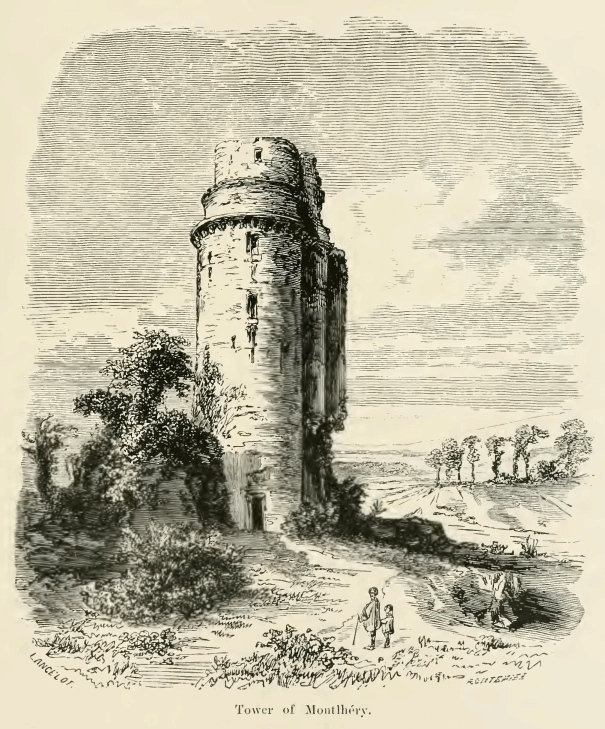
\includegraphics[width=\textwidth]{30191m.jpg}
\end{figure}

“And are you going there?”

“I am.”

“What telegraph do you intend visiting? that of the home department, or
of the observatory?”

“Oh, no; I should find there people who would force me to understand
things of which I would prefer to remain ignorant, and who would try to
explain to me, in spite of myself, a mystery which even they do not
understand. \textit{Ma foi!} I should wish to keep my illusions concerning
insects unimpaired; it is quite enough to have those dissipated which I
had formed of my fellow-creatures. I shall, therefore, not visit either
of these telegraphs, but one in the open country where I shall find a
good-natured simpleton, who knows no more than the machine he is
employed to work.”

“You are a singular man,” said Villefort.

“What line would you advise me to study?”

“The one that is most in use just at this time.”

“The Spanish one, you mean, I suppose?”

“Yes; should you like a letter to the minister that they might explain
to you——”

“No,” said Monte Cristo; “since, as I told you before, I do not wish to
comprehend it. The moment I understand it there will no longer exist a
telegraph for me; it will be nothing more than a sign from M. Duchâtel,
or from M. Montalivet, transmitted to the prefect of Bayonne, mystified
by two Greek words, \textit{têle}, \textit{graphein}. It is the insect with black
claws, and the awful word which I wish to retain in my imagination in
all its purity and all its importance.”

“Go then; for in the course of two hours it will be dark, and you will
not be able to see anything.”

“\textit{Ma foi!} you frighten me. Which is the nearest way? Bayonne?”

“Yes; the road to Bayonne.”

“And afterwards the road to Châtillon?”

“Yes.”

“By the tower of Montlhéry, you mean?”

“Yes.”

“Thank you. Good-bye. On Saturday I will tell you my impressions
concerning the telegraph.”

At the door the count was met by the two notaries, who had just
completed the act which was to disinherit Valentine, and who were
leaving under the conviction of having done a thing which could not
fail of redounding considerably to their credit.
